\documentclass[12pt, a4paper]{article}

\usepackage{amsmath}
\usepackage{booktabs}
\usepackage{ctex}
\usepackage{enumitem}
\usepackage{fancyhdr}
\usepackage{float}
\usepackage{geometry}
\usepackage{graphicx}
\usepackage[colorlinks,linkcolor=black,anchorcolor=black,citecolor=blue,CJKbookmarks=True]{hyperref}
\usepackage{listings}
\usepackage{pifont}
\usepackage{url}
\usepackage{xcolor}

\definecolor{anhao-orange}{RGB}{255,140,0}
\definecolor{anhao-purple}{RGB}{148,0,211}
\definecolor{anhao-scarlet}{RGB}{178,34,34}
\definecolor{anhao-sky}{RGB}{30,144,255}
\definecolor{anhao-background}{RGB}{230,230,250}
\geometry{left=2cm,right=2cm,top=2cm,bottom=2cm}
\renewcommand{\contentsname}{\centering{\heiti\zihao{3}{Contents}}}

\begin{document}
	
\pagenumbering{Roman}
{\tableofcontents}
\newpage

\pagenumbering{arabic}

\section{Lecture 01 - 方程组的几何解释}
\pagestyle{fancy}
\lhead{}
\chead{Lecture 01 - 方程组的几何解释}
\rhead{}

\noindent{\bf{n}} linear equations, {\bf{n}} unknowns
\begin{itemize}
	\item row picture
	\item column picture {\textcolor{anhao-scarlet}{\bf{$\star$}}}
	\item matrix form
\end{itemize}
\vspace{14pt}
\begin{math}
\left\{  
\begin{array}{rclrcl}
	2x & - & y  & = & 0 \\
	-x & + & 2y & = & 3
\end{array}  
\right.
\end{math}
\newline
\begin{math}
\begin{bmatrix}
	2  & -1 \\
	-1 & 2
\end{bmatrix}
\begin{bmatrix}
	x \\
	y
\end{bmatrix}
=
\begin{bmatrix}
	0 \\
	3
\end{bmatrix}
\end{math}
, i.e.
\newline
{\bf{A}} (matrix of coefficients) = 
\begin{math}
\begin{bmatrix}
	2  & -1 \\
	-1 & 2
\end{bmatrix}
\end{math}
, {\bf{x}} (vector of unknowns) = 
\begin{math}
\begin{bmatrix}
	x \\
	y
\end{bmatrix}
\end{math}
, {\bf{b}} = 
\begin{math}
\begin{bmatrix}
	0 \\
	3
\end{bmatrix}
\end{math}
, such that
\begin{displaymath}
{\bf{A}}{\bf{x}}={\bf{b}}
\end{displaymath}
\vspace{14pt}
what's the {\textcolor{anhao-scarlet}{\bf{row}}} picture?
\begin{center}
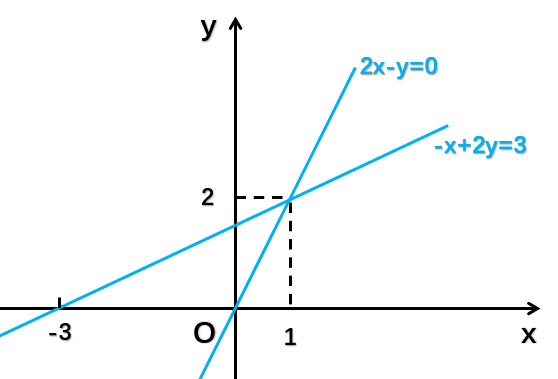
\includegraphics[width=0.4\textwidth]{figures/S1-1.png}
\end{center}
{\textcolor{anhao-purple}{to find the point that lies on both two lines}}
\newline
what's the {\textcolor{anhao-scarlet}{\bf{column}}} picture?
\newline
\begin{math}
x 
\begin{bmatrix}
	2 \\
	-1
\end{bmatrix}
+
y
\begin{bmatrix}
	-1 \\
	2
\end{bmatrix}
=
\begin{bmatrix}
	0 \\
	3
\end{bmatrix}
\end{math}
\begin{center}
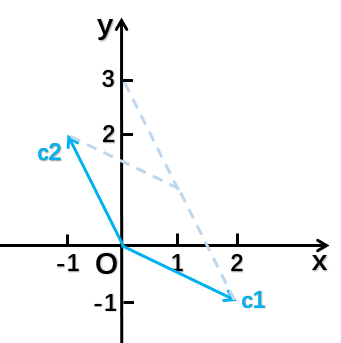
\includegraphics[width=0.3\textwidth]{figures/S1-2.png}
\end{center}
\begin{displaymath}
1{\overrightarrow{c_1}}+2{\overrightarrow{c_2}}={\overrightarrow{b}}
\end{displaymath}
{\textcolor{anhao-purple}{to find the linear combination of columns of {\bf{A}}, such that it equals {\bf{b}}}}
\vspace{14pt}
\newline
what linear combination gives {\bf{b}}?
\newline
what do all the linear combinations give?
\newline
what are all the possible, achievable right-hand sides be?
\vspace{14pt}
\newline
\begin{math}
\left\{  
\begin{array}{rclrclrclrcl}
	2x & - & y & & & = & 0 &{\bf{\textcolor{anhao-orange}{1}}}&\\
	-x & + & 2y & - & z & = & -1 &{\bf{\textcolor{anhao-orange}{2}}}&\\
	& -& 3y & + & 4z & = & 4 &{\bf{\textcolor{anhao-orange}{3}}}&
\end{array}  
\right.
\end{math}
\newline
\begin{math}
\left\{  
\begin{array}{rcl}
	&{\bf{\textcolor{anhao-orange}{1}}}&
\end{array}  
\right.
\end{math}
\quad : the plot of all the points that solve it are a plane
\newline
\begin{math}
\left\{  
\begin{array}{rcl}
	&{\bf{\textcolor{anhao-orange}{2}}}& \\
	&{\bf{\textcolor{anhao-orange}{3}}}&
\end{array}  
\right.
\end{math}
\quad : two planes meet at a line
\newline
\begin{math}
\left\{  
\begin{array}{rcl}
	&{\bf{\textcolor{anhao-orange}{1}}}& \\
	&{\bf{\textcolor{anhao-orange}{2}}}& \\
	&{\bf{\textcolor{anhao-orange}{3}}}&
\end{array}  
\right.
\end{math}
\quad : meet at a point
\newline
{\bf{A}} = 
\begin{math}
\begin{bmatrix}
	2  & -1 & 0 \\
	-1 & 2 & -1 \\
	0 & -3 & 4
\end{bmatrix}
\end{math}
, {\bf{b}} =
\begin{math} 
\begin{bmatrix}
	0 \\
	-1\\
	4
\end{bmatrix}
\end{math}
\vspace{14pt}
\newline
what's the {\textcolor{anhao-scarlet}{\bf{row}}} picture?
\newline
{\textcolor{anhao-purple}{to find out all the points that satisfy all the equations}}
\newline
what's the {\textcolor{anhao-scarlet}{\bf{column}}} picture?
\newline
\begin{math}
x
\begin{bmatrix}
	2 \\
	-1\\
	0
\end{bmatrix}
 + y
\begin{bmatrix}
	-1 \\
	2\\
	-3
\end{bmatrix}
 + z
\begin{bmatrix}
	0 \\
	-1\\
	4
\end{bmatrix}
 = 
\begin{bmatrix}
	0 \\
	-1\\
	4
\end{bmatrix}
\end{math}
\vspace{14pt}
\newline
can I always solve {\bf{A}}{\bf{x}} = {\bf{b}} for every right-hand side {\bf{b}}?
\newline
do the linear combinations of the columns fill 3-dimensional space?
\newline
{\textcolor{anhao-purple}{for this {\bf{A}}, the answer is {\bf{YES}} (non-singular, invertible)}}
\newline
{\textcolor{anhao-purple}{but for some others {\bf{A}}, the answer could be {\bf{NO}} (singular, not-invertible)}}
\vspace{14pt}
\newline
if the 3 columns all lie in the same plane, 
\newline
so I could solve it for some right-hand sides, when ${\overrightarrow{b}}$ is in the plane,
\newline
but most right-hand sides would be out of the plane and unreachable.
\vspace{14pt}
\newline
in some case, the combinations of {\bf{n}} columns can only fill out {\bf{m}}-D (m < n)
\vspace{14pt}
\newline
\begin{math}
\begin{bmatrix}
	2 & 5 \\
	1 & 3 
\end{bmatrix}
\begin{bmatrix}
	1 \\
	2 
\end{bmatrix}
 = 
1
\begin{bmatrix}
	2 \\
	1 
\end{bmatrix}
 + 
2
\begin{bmatrix}
	5 \\
	3 
\end{bmatrix}
 = 
\begin{bmatrix}
	12 \\
	7 
\end{bmatrix}
\end{math}
\newline
{\bf{A}}{\bf{x}} means: {\bf{A}}{\bf{x}} is a combination of columns of {\bf{A}}

\newpage
\section{Lecture 02 - 矩阵消元}
\pagestyle{fancy}
\lhead{}
\chead{Lecture 02 - 矩阵消元}
\rhead{}

\noindent when solving equations-system, 
\newline
{\bf{Elimination}}, if it succeeds, it gets the answer.
\newline
It's always good to ask how could it fail.
\vspace{14pt}
\newline
\begin{math}
	\left\{  
	\begin{array}{rclrclrcl}
		x & + & 2y & + & z & = & 2 \\
		3x & + & 8y & + & z & = & 12 \\
		& & 4y & + & z & = & 2 
	\end{array}  
	\right.
\end{math}
\vspace{14pt}
\newline
\begin{math}
	\begin{bmatrix}
		{\bf{\textcolor{anhao-sky}{\mathop{1}\limits_{first-pivot}}}} & 2 & 1 \\
		3 & 8 & 1 \\
		0 & 4 & 1
	\end{bmatrix}
	\xrightarrow[row_3 - 0 \times row_1]{row_2 - 3 \times row_1}
	\begin{bmatrix}
		1 & 2 & 1 \\
		0 & {\bf{\textcolor{anhao-sky}{\mathop{2}\limits_{second-pivot}}}} & -2 \\
		0 & 4 & 1
	\end{bmatrix}
	\xrightarrow[]{row_3 - 2 \times row_2}
	\begin{bmatrix}
		1 & 2 & 1 \\
		0 & 2 & -2 \\
		0 & 0 & {\bf{\textcolor{anhao-sky}{\mathop{5}\limits_{third-pivot}}}}
	\end{bmatrix}
\end{math}
\newline
{\textcolor{anhao-scarlet}{pivots can {\bf{NOT}} be 0 !}}
\newline
if there is a 0 in the pivot position, then try to switch lines
\newline
if 0 is in the pivot position and no place to exchange, then failure
\vspace{14pt}
\newline
let's bring the right-hand side in (Augmented Matrix)
\newline
\begin{math}
	\left[
	\begin{array}{ccc|c}
		1 & 2 & 1 & 2 \\
		3 & 8 & 1 & 12 \\
		0 & 4 & 1 & 2
	\end{array}
	\right]
	\longrightarrow
	\left[
	\begin{array}{ccc|c}
		1 & 2 & 1 & 2 \\
		0 & 2 & -2 & 6 \\
		0 & 4 & 1 & 2
	\end{array}
	\right]
	\longrightarrow
	\left[
	\begin{array}{ccc|c}
		1 & 2 & 1 & 2 \\
		0 & 2 & -2 & 6 \\
		0 & 0 & 5 & -10
	\end{array}
	\right]
	\Rightarrow
	\left\{  
	\begin{array}{rclrclrcl}
		x & + & 2y & + & z  & = & 2 \\
		  &   & 2y & - & 2z & = & 6  \\
		  &   &    &   & 5z & = & -10  
	\end{array}  
	\right.
\end{math}
\newline
by back-substitution: 
\begin{math}
	x = 2, y = 1, z = -2
\end{math}
\vspace{14pt}
\newline
{\bf{"elimination matrices"}}
\vspace{14pt}
\newline
\begin{math}
	\begin{bmatrix}
		{\textcolor{anhao-orange}{\vdots}} & {\textcolor{green}{\vdots}} & {\textcolor{purple}{\vdots}} \\
		{\textcolor{anhao-orange}{col_1}} & {\textcolor{green}{col_2}} & {\textcolor{purple}{col_3}} \\
		{\textcolor{anhao-orange}{\vdots}} & {\textcolor{green}{\vdots}} & {\textcolor{purple}{\vdots}}
	\end{bmatrix}
	\begin{bmatrix}
		1 \\
		2 \\
		3
	\end{bmatrix}
	 = 
	\begin{bmatrix}
		\ \\
		\ \\
		\ 
	\end{bmatrix}
	 = 
	1 \times {\textcolor{anhao-orange}{col_1}} + 2 \times {\textcolor{green}{col_2}} + 3 \times {\textcolor{purple}{col_3}}
\end{math}
\newline
{\textcolor{anhao-purple}{the result of multiplying a matrix by some vectors, is a combination of columns of the matrix}}
\vspace{14pt}
\newline
\begin{math}
	\begin{bmatrix}
		1 & 2 & 7
	\end{bmatrix}
	\begin{bmatrix}
		{\textcolor{anhao-orange}{\cdots}} & {\textcolor{anhao-orange}{row_1}} & {\textcolor{anhao-orange}{\cdots}} \\
		{\textcolor{green}{\cdots}} & {\textcolor{green}{row_2}} & {\textcolor{green}{\cdots}} \\
		{\textcolor{purple}{\cdots}} & {\textcolor{purple}{row_3}} & {\textcolor{purple}{\cdots}}
	\end{bmatrix}
	 = 
	\begin{bmatrix}
		\ & \ & \
	\end{bmatrix}
	 = 
	\begin{array}{rcl}
		1 & \times &  {\textcolor{anhao-orange}{row_1}} \\
		 & + & \\
		2 & \times & {\textcolor{green}{row_2}} \\
		 & + & \\
		7 & \times & {\textcolor{purple}{row_3}}
	\end{array}
\end{math}
\newline
{\textcolor{anhao-purple}{the product of a row times a matrix, is a combination of rows of the matrix}}
\vspace{14pt}
\newline
when we do matrix multiplication, keep your eye on what it is doing with the whole vectors
\vspace{14pt}
\newline
what does the matrix, which can subtract $3 \times row_1$ from $row_2$ look like?
\newline
i.e. 
\begin{math}
	\begin{bmatrix}
		? & ? & ? \\
		? & ? & ? \\
		? & ? & ? 
	\end{bmatrix}
	\begin{bmatrix}
		1 & 2 & 1 \\
		3 & 8 & 1 \\
		0 & 4 & 1 
	\end{bmatrix}
	 = 
	\begin{bmatrix}
		1 & 2 & 1 \\
		0 & 2 & -2 \\
		0 & 4 & 1 
	\end{bmatrix}
\end{math}
\newline
\begin{math}
	\begin{bmatrix}
		? & ? & ? \\
		? & ? & ? \\
		? & ? & ? 
	\end{bmatrix}
	\\
	\xrightarrow[]{as \ R_1 = {\textcolor{anhao-scarlet}{\bf{1}}} \times row_1 + {\textcolor{anhao-scarlet}{\bf{0}}} \times row_2 + {\textcolor{anhao-scarlet}{\bf{0}}} \times row_3}
	\begin{bmatrix}
		1 & 0 & 0 \\
		? & ? & ? \\
		? & ? & ? 
	\end{bmatrix}
	\\
	\xrightarrow[]{as \ R_3 = {\textcolor{anhao-scarlet}{\bf{0}}} \times row_1 + {\textcolor{anhao-scarlet}{\bf{0}}} \times row_2 + {\textcolor{anhao-scarlet}{\bf{1}}} \times row_3}
	\begin{bmatrix}
		1 & 0 & 0 \\
		? & ? & ? \\
		0 & 0 & 1 
	\end{bmatrix}
	\\
	\xrightarrow[]{as \ R_2 = {\textcolor{anhao-scarlet}{\bf{-3}}} \times row_1 + {\textcolor{anhao-scarlet}{\bf{1}}} \times row_2 + {\textcolor{anhao-scarlet}{\bf{0}}} \times row_3}
	\begin{bmatrix}
		1 & 0 & 0 \\
		-3 & 1 & 0 \\
		0 & 0 & 1 
	\end{bmatrix}
\end{math}
\newline
\begin{math}
	\begin{bmatrix}
		1 & 0 & 0 \\
		-3 & 1 & 0 \\
		0 & 0 & 1 
	\end{bmatrix}
\end{math}
: elementary matrix (初等矩阵)
\newline
${\bf{E_{i,j}}}$ means it's the matrix that we use to fix the (i, j) position
\newline
e.g. 
\begin{math}
	\begin{bmatrix}
		? & ? & ? \\
		? & ? & ? \\
		? & ? & ? 
	\end{bmatrix}
	\xrightarrow[]{R_1=row_1}
	\begin{bmatrix}
		1 & 0 & 0 \\
		? & ? & ? \\
		? & ? & ? 
	\end{bmatrix}
	\xrightarrow[]{R_2=row_2}
	\begin{bmatrix}
		1 & 0 & 0 \\
		0 & 1 & 0 \\
		? & ? & ? 
	\end{bmatrix}
	\xrightarrow[]{R_3 = row_3 - 2 \times row_2}
	\begin{bmatrix}
		1 & 0 & 0 \\
		0 & 1 & 0 \\
		0 & -2 & 1 
	\end{bmatrix}
	 = 
	E_{3,2}
\end{math}
\vspace{14pt}
\newline
in elimination, we can use an elementary matrix to describe the change in each step
\vspace{14pt}
\newline
the next point in this lecture is to put these steps together, into a matrix that does these steps all in sequence, in another words, how could I create the matrix that does the whole job at once? i.e.
\begin{displaymath}
	{\bf{E_{3,2}}}({\bf{E_{2,1}}}{\bf{A}}) = {\bf{U}} \Longleftrightarrow {\bf{\boxed{?}}}{\bf{A}} = {\bf{U}}
\end{displaymath}
\vspace{14pt}
\newline
{\bf{Associative Law}}
\begin{displaymath}
	({\bf{A}}{\bf{B}}){\bf{C}} = {\bf{A}}({\bf{B}}{\bf{C}})
\end{displaymath}
\vspace{14pt}
\newline
permutation(置换): 
\begin{itemize}
	\item exchange rows, e.g.
	\par 
	\begin{math}
		\begin{bmatrix}
			? & ? \\
			? & ?
		\end{bmatrix}
		\begin{bmatrix}
			a & b \\
			c & d
		\end{bmatrix}
		 = 
		\begin{bmatrix}
			c & d \\
			a & b
		\end{bmatrix}
	\end{math}
	\par {\bf{P}} = 
	\begin{math}
		\begin{bmatrix}
			0 & 1 \\
			1 & 0
		\end{bmatrix}
	\end{math}
	is to exchange $row_1$ and $row_2$
	\item exchange columns, e.g.
	\par 
	\begin{math}
		\begin{bmatrix}
			a & b \\
			c & d
		\end{bmatrix}
		\begin{bmatrix}
			? & ? \\
			? & ?
		\end{bmatrix}
		= 
		\begin{bmatrix}
			b & a \\
			d & c
		\end{bmatrix}
	\end{math}
	\par {\bf{P}} = 
	\begin{math}
		\begin{bmatrix}
			0 & 1 \\
			1 & 0
		\end{bmatrix}
	\end{math}
	is to exchange $col_1$ and $col_2$
\end{itemize}
\vspace{14pt}
{\textcolor{anhao-purple}{when I multiply a matrix on the left, I am doing row operations}}
\newline
{\textcolor{anhao-purple}{if I want to do column operations, I should put a matrix on the right}}
\vspace{14pt}
\newline
if ${\bf{\boxed{?}}}{\bf{A}} = {\bf{U}}$, then how can I "from {\bf{U}} back to {\bf{A}}"?
\newline
this is about reversing steps, invertible, $\cdots$
\newline
\begin{math}
	\begin{bmatrix}
		1 & 0 & 0 \\
		-3 & 1 & 0 \\
		0 & 0 & 1
	\end{bmatrix}^{-1}
	 = 
	\begin{bmatrix}
		1 & 0 & 0 \\
		3 & 1 & 0 \\
		0 & 0 & 1
	\end{bmatrix}
\end{math}
\newline
"what steps can get me back?"
\newline
"what matrix can bring me back?"

\newpage
\section{Lecture 03 - 乘法和逆矩阵}
\pagestyle{fancy}
\lhead{}
\chead{Lecture 03 - 乘法和逆矩阵}
\rhead{}


\end{document}